\chapter{Xray Architecture and Integration with Smart Relay}

This chapter provides a comprehensive analysis of Xray-core's internal architecture, how it processes connections, and how the Smart Relay Rust client integrates with it. We cover the complete lifecycle from configuration generation to connection routing, with detailed diagrams and code examples.

\section{Xray-Core Architecture Overview}

Xray-core is built on a modular, feature-based architecture where components are registered as \textbf{Features} and managed through dependency injection. The core instance orchestrates all features and handles their lifecycle.

\subsection{Core Components}

Xray's architecture consists of several key components:

\begin{itemize}
    \item \textbf{Instance}: The main Xray server instance that manages all features
    \item \textbf{Features}: Modular components (DNS, Routing, Inbound/Outbound Managers, etc.)
    \item \textbf{Inbound Handlers}: Accept connections from clients (SOCKS5, HTTP proxy)
    \item \textbf{Outbound Handlers}: Establish connections to VPN servers (VMess, VLESS, Shadowsocks)
    \item \textbf{Dispatcher}: Routes traffic between inbounds and outbounds
    \item \textbf{Router}: Makes routing decisions based on rules
    \item \textbf{DNS Client}: Resolves domain names
\end{itemize}

\begin{figure}[h]
    \centering
    \begin{tikzpicture}[node distance=3cm,>=stealth,thick]
        \node (instance) [draw, rectangle, minimum width=3cm, minimum height=2cm, fill=blue!20] {Xray Instance};
        
        \node (inbound) [draw, rectangle, minimum width=2.5cm, minimum height=1.5cm, left of=instance, xshift=-2cm, fill=green!20] {Inbound Manager};
        \node (outbound) [draw, rectangle, minimum width=2.5cm, minimum height=1.5cm, right of=instance, xshift=2cm, fill=red!20] {Outbound Manager};
        \node (dns) [draw, rectangle, minimum width=2.5cm, minimum height=1.5cm, below of=instance, yshift=-1cm, fill=purple!20] {DNS Client};
        \node (dispatcher) [draw, rectangle, minimum width=2.5cm, minimum height=1.5cm, above of=router, yshift=0.5cm, fill=orange!20] {Dispatcher};
        \node (router) [draw, rectangle, minimum width=2.5cm, minimum height=1.5cm, left of=dispatcher, xshift=-2cm, fill=yellow!20] {Router};

        \draw[<->] (instance) -- (inbound);
        \draw[<->] (instance) -- (outbound);
        \draw[<->] (instance) -- (router);
        \draw[<->] (instance) -- (dns);
        \draw[<->] (instance) -- (dispatcher);
        \draw[->] (dispatcher) -- (router);
        \draw[->] (router) -- (outbound);
        \draw[->] (inbound) -- (dispatcher);
    \end{tikzpicture}
    \caption{Xray-Core Architecture: Feature-Based Modular Design}
\end{figure}

\subsection{Instance Initialization}

The Xray Instance is created from a configuration object. During initialization:

\begin{enumerate}
    \item \textbf{Feature Registration}: All features (DNS, Router, Inbound/Outbound Managers) are registered
    \item \textbf{Dependency Resolution}: Features with dependencies wait until dependencies are available
    \item \textbf{Handler Creation}: Inbound and outbound handlers are created from configuration
    \item \textbf{System Initialization}: DNS client and system dialer are initialized
\end{enumerate}

\begin{verbatim}
// From Xray-core: core/xray.go
func New(config *Config) (*Instance, error) {
    server := &Instance{ctx: context.Background()}
    
    // Register all features from config
    for _, appSettings := range config.App {
        settings, err := appSettings.GetInstance()
        if err != nil {
            return nil, err
        }
        obj, err := CreateObject(server, settings)
        if err != nil {
            return nil, err
        }
        if feature, ok := obj.(features.Feature); ok {
            if err := server.AddFeature(feature); err != nil {
                return nil, err
            }
        }
    }
    
    // Add essential features if not present
    essentialFeatures := []struct {
        Type     interface{}
        Instance features.Feature
    }{
        {dns.ClientType(), localdns.New()},
        {policy.ManagerType(), policy.DefaultManager{}},
        {routing.RouterType(), routing.DefaultRouter{}},
        {stats.ManagerType(), stats.NoopManager{}},
    }
    
    // Initialize inbounds and outbounds
    if err := addInboundHandlers(server, config.Inbound); err != nil {
        return nil, err
    }
    
    if err := addOutboundHandlers(server, config.Outbound); err != nil {
        return nil, err
    }
    
    return server, nil
}
\end{verbatim}

\section{Smart Relay Rust Client Integration}

The Smart Relay Rust client manages Xray as an external process, communicating through configuration files and monitoring the process lifecycle.

\subsection{XrayAdapter Structure}

The \texttt{XrayAdapter} struct manages the Xray process and configuration:

\begin{verbatim}
// From Smart Relay: src/proxy/xray_adapter.rs
pub struct XrayAdapter {
    xray_path: PathBuf,              // Path to xray.exe binary
    process: Arc<Mutex<Option<Child>>>,  // Xray process handle
    config_path: PathBuf,            // Path to config JSON file
    socks_port: u16,                  // Configured SOCKS5 port
    http_port: u16,                   // Configured HTTP proxy port
    api_port: u16,                    // API port (for future use)
    actual_socks_port: Arc<Mutex<Option<u16>>>,  // Actual port (after fallback)
    actual_http_port: Arc<Mutex<Option<u16>>>,  // Actual port (after fallback)
}
\end{verbatim}

\subsection{Configuration Generation Flow}

The Rust client generates Xray configuration from endpoint data:

\begin{figure}[h]
    \centering
    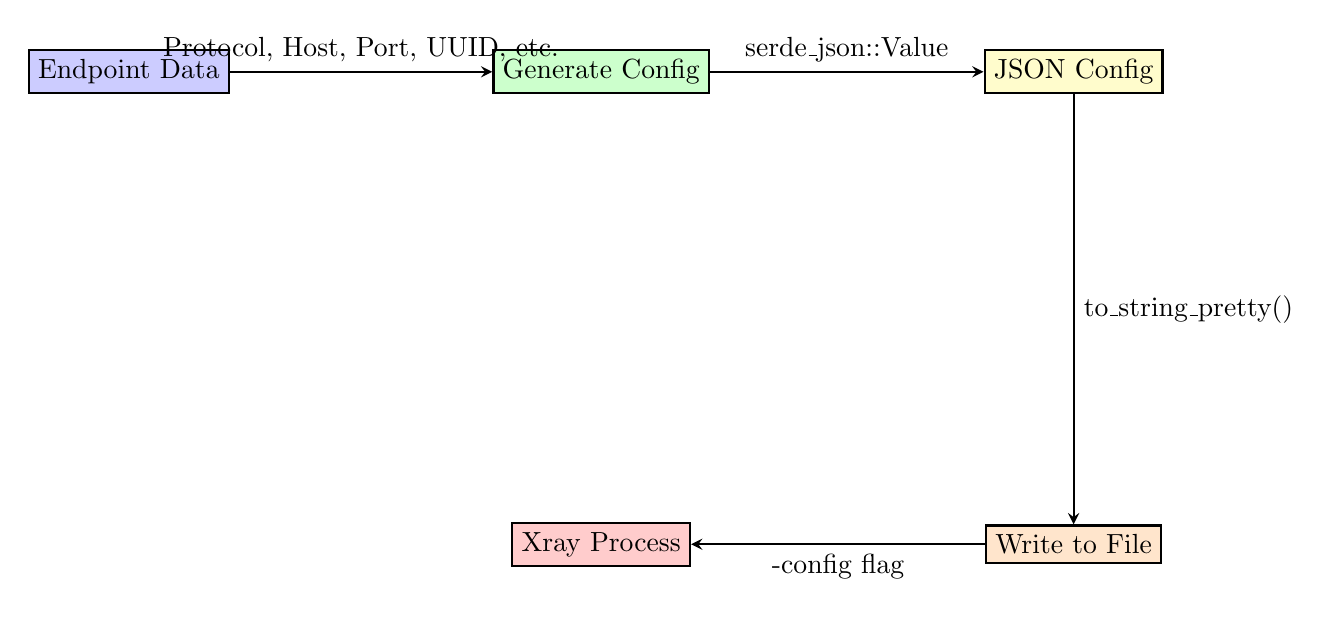
\begin{tikzpicture}[node distance=6cm,>=stealth,thick]
        \node (endpoint) [draw, rectangle, fill=blue!20] {Endpoint Data};
        \node (config) [draw, rectangle, right of=endpoint, fill=green!20] {Generate Config};
        \node (json) [draw, rectangle, right of=config, fill=yellow!20] {JSON Config};
        \node (file) [draw, rectangle, below of=json, fill=orange!20] {Write to File};
        \node (xray) [draw, rectangle, left of=file, fill=red!20] {Xray Process};
        
        \draw[->] (endpoint) -- node[above] {Protocol, Host, Port, UUID, etc.} (config);
        \draw[->] (config) -- node[above] {serde\_json::Value} (json);
        \draw[->] (json) -- node[right] {to\_string\_pretty()} (file);
        \draw[->] (file) -- node[below] {-config flag} (xray);
    \end{tikzpicture}
    \caption{Configuration Generation and Passing to Xray}
\end{figure}

\subsubsection{Configuration Generation Code}

\begin{verbatim}
// From Smart Relay: src/proxy/xray_adapter.rs
pub fn generate_config(&self, endpoint: &EndpointConfig) -> Result<Value> {
    // Generate outbound based on protocol
    let mut outbound = match endpoint.protocol.to_lowercase().as_str() {
        "vmess" => self.generate_vmess_outbound(endpoint)?,
        "vless" => self.generate_vless_outbound(endpoint)?,
        "shadowsocks" => self.generate_shadowsocks_outbound(endpoint)?,
        "trojan" => self.generate_trojan_outbound(endpoint)?,
        "socks5" => self.generate_socks5_outbound(endpoint)?,
        _ => return Err(anyhow::anyhow!("Unsupported protocol")),
    };
    
    outbound["tag"] = json!("proxy");
    
    // Build complete configuration
    let config = json!({
        "log": { "loglevel": "warning" },
        "inbounds": [
            {
                "port": socks_port,
                "protocol": "socks",
                "settings": { "auth": "noauth", "udp": true },
                "sniffing": { "enabled": true, "destOverride": ["http", "tls"] }
            },
            {
                "port": http_port,
                "protocol": "http",
                "settings": { "allowTransparent": false }
            }
        ],
        "outbounds": [
            outbound,
            { "protocol": "freedom", "tag": "direct" },
            { "protocol": "blackhole", "tag": "blocked" }
        ],
        "routing": {
            "domainStrategy": "IPOnDemand",
            "rules": [
                {
                    "type": "field",
                    "network": "tcp,udp",
                    "outboundTag": "proxy"
                }
            ]
        }
    });
    
    Ok(config)
}
\end{verbatim}

\subsection{Process Lifecycle Management}

\subsubsection{Starting Xray}

The Rust client starts Xray with careful port management and error handling:

\begin{verbatim}
// From Smart Relay: src/proxy/xray_adapter.rs
pub fn start(&self) -> Result<()> {
    let mut process_guard = self.process.lock().unwrap();
    
    if process_guard.is_some() {
        warn!("Xray is already running");
        return Ok(());
    }
    
    // Check port availability with retries
    let max_retries = 5;
    for attempt in 0..max_retries {
        let (socks_avail, http_avail) = check_ports_available_sync(
            self.socks_port, 
            self.http_port
        );
        
        if socks_avail && http_avail {
            break;
        }
        
        if attempt < max_retries - 1 {
            // Try to kill processes using ports
            let _ = self.kill_processes_using_ports();
            std::thread::sleep(Duration::from_millis(500 * (attempt + 1)));
        } else {
            // Find alternative ports
            let (alt_socks, alt_http) = find_available_ports_sync()?;
            // Update config with alternative ports
            // ...
        }
    }
    
    // Spawn Xray process
    let child = Command::new(&self.xray_path)
        .arg("-config")
        .arg(&self.config_path)
        .stdout(Stdio::piped())
        .stderr(Stdio::piped())
        .spawn()
        .context("Failed to start xray process")?;
    
    let pid = child.id();
    *process_guard = Some(child);
    
    // Wait for initialization
    std::thread::sleep(Duration::from_millis(1000));
    
    // Check if process exited immediately (port binding error)
    // If so, retry with alternative ports
    
    Ok(())
}
\end{verbatim}

\subsubsection{Stopping Xray}

\begin{verbatim}
// From Smart Relay: src/proxy/xray_adapter.rs
pub fn stop(&self) -> Result<()> {
    let mut process_guard = self.process.lock().unwrap();
    
    if let Some(mut child) = process_guard.take() {
        let pid = child.id();
        
        // On Windows, kill process tree
        #[cfg(windows)]
        {
            let _ = Command::new("taskkill")
                .args(&["/F", "/T", "/PID", &pid.to_string()])
                .output();
            let _ = child.kill();
        }
        
        // Wait for process to exit with timeout
        let start = std::time::Instant::now();
        loop {
            match child.try_wait() {
                Ok(Some(_)) => break,
                Ok(None) => {
                    if start.elapsed().as_secs() > 5 {
                        let _ = child.kill();
                        let _ = child.wait();
                        break;
                    }
                    std::thread::sleep(Duration::from_millis(100));
                }
                Err(e) => {
                    warn!("Error waiting for Xray: {}", e);
                    break;
                }
            }
        }
        
        // Wait for ports to be released
        // ...
    }
    
    Ok(())
}
\end{verbatim}

\section{Connection Flow: Client to VPN Server}

Understanding how connections flow through Xray is crucial for debugging and optimization.

\subsection{Complete Connection Path}

\begin{figure}[h]
    \centering
    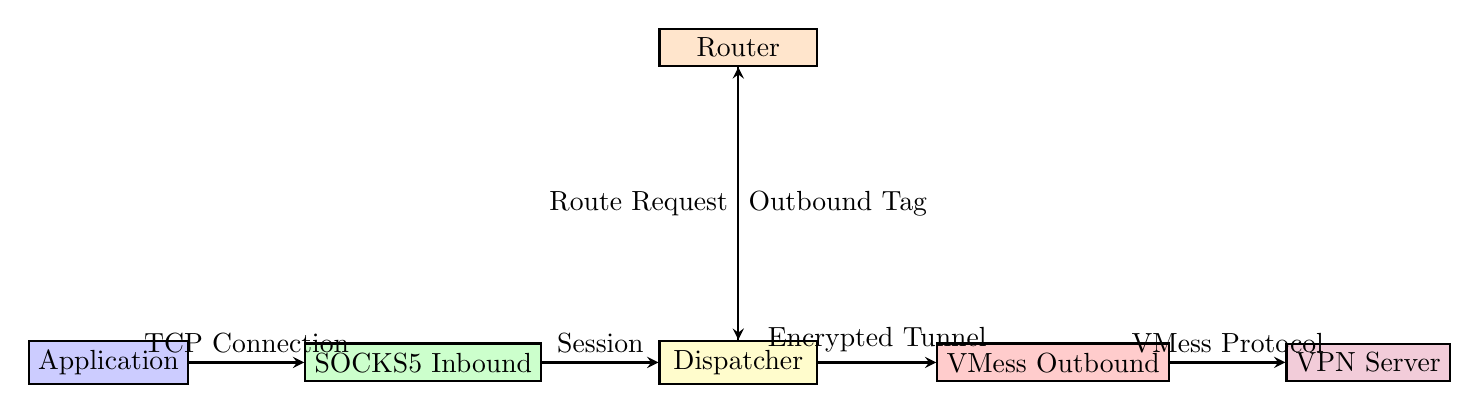
\begin{tikzpicture}[node distance=4cm,>=stealth,thick]
        \node (app) [draw, rectangle, fill=blue!20, minimum width=2cm] {Application};
        \node (socks) [draw, rectangle, right of=app, fill=green!20, minimum width=2cm] {SOCKS5 Inbound};
        \node (dispatcher) [draw, rectangle, right of=socks, fill=yellow!20, minimum width=2cm] {Dispatcher};
        \node (router) [draw, rectangle, above of=dispatcher, fill=orange!20, minimum width=2cm] {Router};
        \node (outbound) [draw, rectangle, right of=dispatcher, fill=red!20, minimum width=2cm] {VMess Outbound};
        \node (server) [draw, rectangle, right of=outbound, fill=purple!20, minimum width=2cm] {VPN Server};
        
        \draw[->] (app) -- node[above] {TCP Connection} (socks);
        \draw[->] (socks) -- node[above] {Session} (dispatcher);
        \draw[->] (dispatcher) -- node[left] {Route Request} (router);
        \draw[->] (router) -- node[right] {Outbound Tag} (dispatcher);
        \draw[->] (dispatcher) -- node[above] {Encrypted Tunnel} (outbound);
        \draw[->] (outbound) -- node[above] {VMess Protocol} (server);
    \end{tikzpicture}
    \caption{Complete Connection Flow Through Xray}
\end{figure}

\subsection{Step-by-Step Connection Processing}

\subsubsection{Step 1: Inbound Handler Accepts Connection}

When a client connects to the SOCKS5 port (e.g., 127.0.0.1:1080):

\begin{verbatim}
// Xray inbound handler accepts connection
// From Xray-core: app/proxyman/inbound/inbound.go
func (m *Manager) AddHandler(ctx context.Context, handler inbound.Handler) error {
    // Handler starts listening on configured port
    if m.running {
        return handler.Start()  // Begin accepting connections
    }
    return nil
}
\end{verbatim}

The SOCKS5 handler:
\begin{enumerate}
    \item Accepts TCP connection on port 1080
    \item Performs SOCKS5 handshake (authentication, command, address)
    \item Creates a \textbf{Session} object with destination information
    \item Passes session to the Dispatcher
\end{enumerate}

\subsubsection{Step 2: Dispatcher Receives Session}

The Dispatcher is the central routing component:

\begin{verbatim}
// From Xray-core: app/dispatcher/dispatcher.go
// The dispatcher receives a session and:
// 1. Extracts destination (IP/port or domain)
// 2. Calls Router to determine outbound
// 3. Forwards session to appropriate outbound handler
\end{verbatim}

\subsubsection{Step 3: Router Makes Routing Decision}

The Router evaluates rules to determine which outbound to use:

\begin{verbatim}
// From Xray-core: app/router/router.go
func (r *Router) PickRoute(ctx routing.Context) (routing.Route, error) {
    // Evaluate rules in order
    for _, rule := range r.rules {
        if rule.Condition.Apply(ctx) {
            // Rule matches, return associated outbound tag
            return &Route{
                outboundTag: rule.Tag,
                ruleTag: rule.RuleTag,
            }, nil
        }
    }
    
    // Default: use first outbound or direct
    return defaultRoute, nil
}
\end{verbatim}

Routing rules can match on:
\begin{itemize}
    \item \textbf{Domain}: Specific domains or patterns (e.g., \texttt{geosite:google})
    \item \textbf{IP Address}: IP ranges or GeoIP (e.g., \texttt{geoip:private})
    \item \textbf{Port}: Specific ports or ranges
    \item \textbf{Network}: TCP, UDP, or both
    \item \textbf{Source}: Source IP or tag
\end{itemize}

\subsubsection{Step 4: Outbound Handler Establishes Connection}

Once the router determines the outbound (e.g., \texttt{tag: "proxy"}), the dispatcher forwards the session to the VMess outbound handler:

\begin{verbatim}
// From Xray-core: proxy/vmess/outbound/outbound.go
// The VMess outbound handler:
// 1. Extracts destination from session
// 2. Performs VMess handshake with server:
//    - Generates authentication header (UUID, timestamp, alterId)
//    - Encrypts with ChaCha20-Poly1305 or AES-128-GCM
//    - Sends request header
// 3. Establishes encrypted tunnel
// 4. Forwards application data through tunnel
\end{verbatim}

\subsection{VMess Handshake Details}

The VMess protocol handshake involves several cryptographic operations:

\begin{enumerate}
    \item \textbf{Authentication Header Generation}:
    \[
    \text{Header} = \text{Encrypt}(\text{UUID} || \text{Timestamp} || \text{Nonce}, K)
    \]
    where $K$ is derived from the UUID and server key.
    
    \item \textbf{Request Header}:
    \begin{itemize}
        \item Version (1 byte)
        \item IV (16 bytes, random)
        \item Key (16 bytes, encrypted with server public key)
        \item V (1 byte, response authentication)
        \item Option (1 byte)
        \item Padding (variable)
        \item Command (1 byte: TCP, UDP, Mux)
        \item Port (2 bytes, big-endian)
        \item Address Type (1 byte) + Address (variable)
        \item Random bytes (variable, for padding)
    \end{itemize}
    
    \item \textbf{Response Header}:
    \begin{itemize}
        \item Response (1 byte)
        \item Option (1 byte)
        \item Command (1 byte)
        \item Port (2 bytes)
        \item Address Type + Address
    \end{itemize}
    
    \item \textbf{Data Transmission}:
    After handshake, all data is encrypted using the negotiated key and IV.
\end{enumerate}

\section{Xray Internal Data Structures}

\subsection{Session Object}

The Session object carries connection metadata through Xray:

\begin{verbatim}
// From Xray-core: common/session/session.go
type Session struct {
    ID          ID              // Unique session identifier
    User        *protocol.User  // User associated with connection
    Content     *Content        // Request content (destination, etc.)
    Inbound     *Inbound        // Inbound handler info
    Outbound    *Outbound       // Outbound handler info
    Time        time.Time       // Connection time
}
\end{verbatim}

\subsection{Content Object}

The Content object contains destination information:

\begin{verbatim}
type Content struct {
    Protocol    string          // Protocol (HTTP, TLS, etc.)
    SniffedProtocol string     // Sniffed protocol
    Domain      string          // Destination domain
    Attributes  map[string]string  // Additional attributes
}
\end{verbatim}

\section{Integration Points: Rust Client and Xray}

\subsection{Configuration File Communication}

The Rust client and Xray communicate exclusively through a JSON configuration file:

\begin{enumerate}
    \item \textbf{Rust Client}: Generates JSON config from endpoint data
    \item \textbf{File System}: Writes config to \texttt{xray\_config.json}
    \item \textbf{Xray Process}: Reads config on startup via \texttt{-config} flag
    \item \textbf{No Runtime Communication}: Xray does not accept runtime config changes (must restart)
\end{enumerate}

\begin{figure}[h]
    \centering
    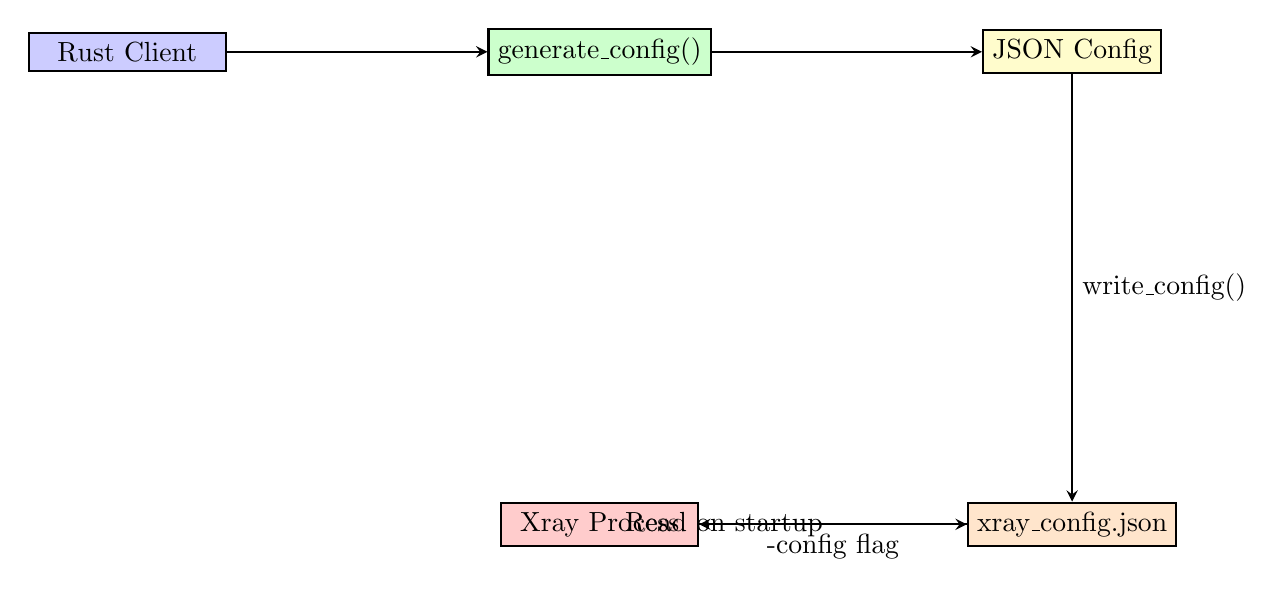
\begin{tikzpicture}[node distance=6cm,>=stealth,thick]
        \node (rust) [draw, rectangle, fill=blue!20, minimum width=2.5cm] {Rust Client};
        \node (gen) [draw, rectangle, right of=rust, fill=green!20, minimum width=2cm] {generate\_config()};
        \node (json) [draw, rectangle, right of=gen, fill=yellow!20, minimum width=2cm] {JSON Config};
        \node (file) [draw, rectangle, below of=json, fill=orange!20, minimum width=2cm] {xray\_config.json};
        \node (xray) [draw, rectangle, left of=file, fill=red!20, minimum width=2.5cm] {Xray Process};
        
        \draw[->] (rust) -- (gen);
        \draw[->] (gen) -- (json);
        \draw[->] (json) -- node[right] {write\_config()} (file);
        \draw[->] (file) -- node[below] {-config flag} (xray);
        \draw[->, dashed] (xray) -- node[left] {Read on startup} (file);
    \end{tikzpicture}
    \caption{Configuration Communication: File-Based}
\end{figure}

\subsection{Process Monitoring}

The Rust client monitors Xray's process status:

\begin{verbatim}
// From Smart Relay: src/proxy/xray_adapter.rs
pub fn is_running(&self) -> bool {
    let process_guard = self.process.lock().unwrap();
    if let Some(ref child) = *process_guard {
        match child.try_wait() {
            Ok(None) => true,   // Process still running
            Ok(Some(_)) => false,  // Process exited
            Err(_) => false,
        }
    } else {
        false
    }
}
\end{verbatim}

\subsection{Port Management}

The Rust client manages ports carefully to avoid conflicts:

\begin{enumerate}
    \item \textbf{Pre-Start Check}: Verifies ports are available before starting Xray
    \item \textbf{Retry Logic}: Retries with delays to handle TIME\_WAIT states
    \item \textbf{Process Killing}: Kills processes using ports if needed (Windows: PowerShell/taskkill)
    \item \textbf{Port Fallback}: Finds alternative ports if configured ports are unavailable
    \item \textbf{Post-Stop Verification}: Waits for ports to be released after stopping Xray
\end{enumerate}

\section{Connection Routing in Detail}

\subsection{Domain Strategy}

Xray supports multiple domain resolution strategies:

\begin{itemize}
    \item \textbf{AsIs}: Use domain as-is, resolve when needed
    \item \textbf{UseIP}: Resolve domain to IP before routing
    \item \textbf{UseIPv4}: Prefer IPv4, fallback to IPv6
    \item \textbf{UseIPv6}: Prefer IPv6, fallback to IPv4
    \item \textbf{IPIfNonMatch}: Resolve to IP if no domain rule matches
    \item \textbf{IPOnDemand}: Resolve on demand (used by Smart Relay)
\end{itemize}

\subsection{Routing Rule Evaluation}

Rules are evaluated in order until a match is found:

\begin{verbatim}
// Example routing configuration from Smart Relay
{
    "routing": {
        "domainStrategy": "IPOnDemand",
        "rules": [
            {
                "type": "field",
                "ip": ["geoip:private"],
                "outboundTag": "direct"
            },
            {
                "type": "field",
                "domain": ["geosite:ads"],
                "outboundTag": "blocked"
            },
            {
                "type": "field",
                "network": "tcp,udp",
                "outboundTag": "proxy"
            }
        ]
    }
}
\end{verbatim}

Evaluation order:
\begin{enumerate}
    \item Check IP rules (geoip:private) → route to "direct" if match
    \item Check domain rules (geosite:ads) → route to "blocked" if match
    \item Check network rules (tcp,udp) → route to "proxy" (catch-all)
\end{enumerate}

\section{Error Handling and Recovery}

\subsection{Port Binding Errors}

When Xray fails to bind to a port:

\begin{enumerate}
    \item \textbf{Detection}: Process exits immediately after spawn
    \item \textbf{Error Reading}: Read stderr to get error message
    \item \textbf{Port Fallback}: Find alternative ports
    \item \textbf{Config Update}: Update JSON config with new ports
    \item \textbf{Retry}: Spawn Xray again with new ports
\end{enumerate}

\begin{verbatim}
// From Smart Relay: src/proxy/xray_adapter.rs
if process_exited {
    // Read error output
    let error_output = read_xray_output(&mut process_guard_check)?;
    
    if error_output.contains("bind:") || error_output.contains("address already in use") {
        // Port binding error, find alternatives
        let (alt_socks, alt_http) = find_available_ports_sync()?;
        // Update config and retry
    }
}
\end{verbatim}

\subsection{Connection Failures}

When connections fail:

\begin{enumerate}
    \item \textbf{Local Proxy Check}: Verify SOCKS5/HTTP ports are listening
    \item \textbf{DNS Resolution}: Check if destination domain resolves
    \item \textbf{Direct Connection Test}: Test TCP connection to VPN server
    \item \textbf{Routing Check}: Verify routing rules are correct
    \item \textbf{Protocol Errors}: Check VMess/VLESS configuration (UUID, time sync, etc.)
\end{enumerate}

\section{Performance Considerations}

\subsection{Connection Pooling}

Xray maintains connection pools for outbound handlers to reuse connections:

\begin{itemize}
    \item \textbf{VMess}: Reuses connections when possible (same server, same user)
    \item \textbf{VLESS}: Connection reuse with session tickets
    \item \textbf{Shadowsocks}: Simple connection reuse
\end{itemize}

\subsection{Memory Management}

Xray uses buffer pools to reduce allocations:

\begin{verbatim}
// From Xray-core: common/buf/buf.go
// Buffers are pooled and reused to reduce GC pressure
type Buffer struct {
    v []byte
    // ...
}
\end{verbatim}

\subsection{Concurrency}

Xray handles connections concurrently:
\begin{itemize}
    \item Each inbound connection is handled in a separate goroutine
    \item Outbound connections are established asynchronously
    \item Routing decisions are made without blocking
\end{itemize}

\section{Summary}

This chapter covered:

\begin{itemize}
    \item \textbf{Xray Architecture}: Feature-based modular design with Instance, Features, Managers
    \item \textbf{Rust Client Integration}: XrayAdapter manages process lifecycle and configuration
    \item \textbf{Configuration Flow}: JSON config generation → file write → Xray startup
    \item \textbf{Connection Flow}: Application → Inbound → Dispatcher → Router → Outbound → VPN Server
    \item \textbf{Routing}: Rule-based routing with domain/IP/network matching
    \item \textbf{Error Handling}: Port management, connection failures, recovery strategies
    \item \textbf{Performance}: Connection pooling, buffer management, concurrency
\end{itemize}

Understanding this architecture is essential for:
\begin{itemize}
    \item Debugging connection issues
    \item Optimizing performance
    \item Implementing new features
    \item Integrating with other systems
\end{itemize}

